\subsection{Synthetic Tests for Vertical Stripes in the 16-Code Matched Filter}
\label{app:head-vertical-stripe-simulation}

The raw Clinton range--Doppler patch in Fig.~\ref{fig:head-gaussian-example}
contains weak nearly vertical structures with a spacing associated with the
100 Hz repeated-code ambiguity.  To test whether these stripes are an intrinsic
consequence of the 16-code coherent processing, the same matched-filter grid was
recomputed with synthetic voltage data.  The simulation used the Clinton code
length, interpolation factor, 16-code coherent window, Doppler bins, and range
gates of the 0.400 s example.  A single point-like head echo was inserted at
263.25 km and -2175.0 Hz,
with the target amplitude adjusted so that the peak-to-median contrast of the
synthetic matched-filter image matched the observed raw patch
(20.4 dB).

Figure~\ref{fig:head-vertical-stripe-simulation} compares the observed raw
patch with several synthetic variants.  The first simulation uses one transmit
code, one matched code, and one receiver channel.  The following simulations add
the second receiver channel and then all five simultaneously transmitted code
seeds used in the experiment.  The final panel is a deliberately crude stress
test in which a strong zero-Doppler code-like leakage term is added; it is not a
physical direct-path model, but it tests whether stationary code leakage can
produce coherent Doppler-column structure.

\begin{table}[h]
  \centering
  \caption{Image-frequency power in the 100 Hz comb columns for the synthetic
  Clinton vertical-stripe tests.  Values are the mean two-dimensional Fourier
  power in the repeated-code comb columns relative to the mean power outside
  those columns.  The same statistic is listed before and after the 2-D FFT
  notch used for the micro-Doppler diagnostic.
  \figsource{reports/simulate_head_echo_vertical_stripes.py}}
  \begin{tabular}{lrr}
    \toprule
    Simulation & Raw comb/off (dB) & Notched comb/off (dB) \\
    \midrule
Observed Clinton raw patch & 28.5 & -289.4 \\
1 TX code, 1 RX channel & -0.0 & -300.0 \\
1 TX code, 2 RX channels & 0.1 & -300.0 \\
5 TX codes, equal phases & 7.0 & -296.2 \\
5 TX codes, random phases & 7.1 & -296.3 \\
5 TX + strong zero-Doppler leakage & 29.3 & -296.9 \\
    \bottomrule
  \end{tabular}
  \label{tab:head-vertical-stripe-simulation}
\end{table}

\begin{figure}
  \centering
  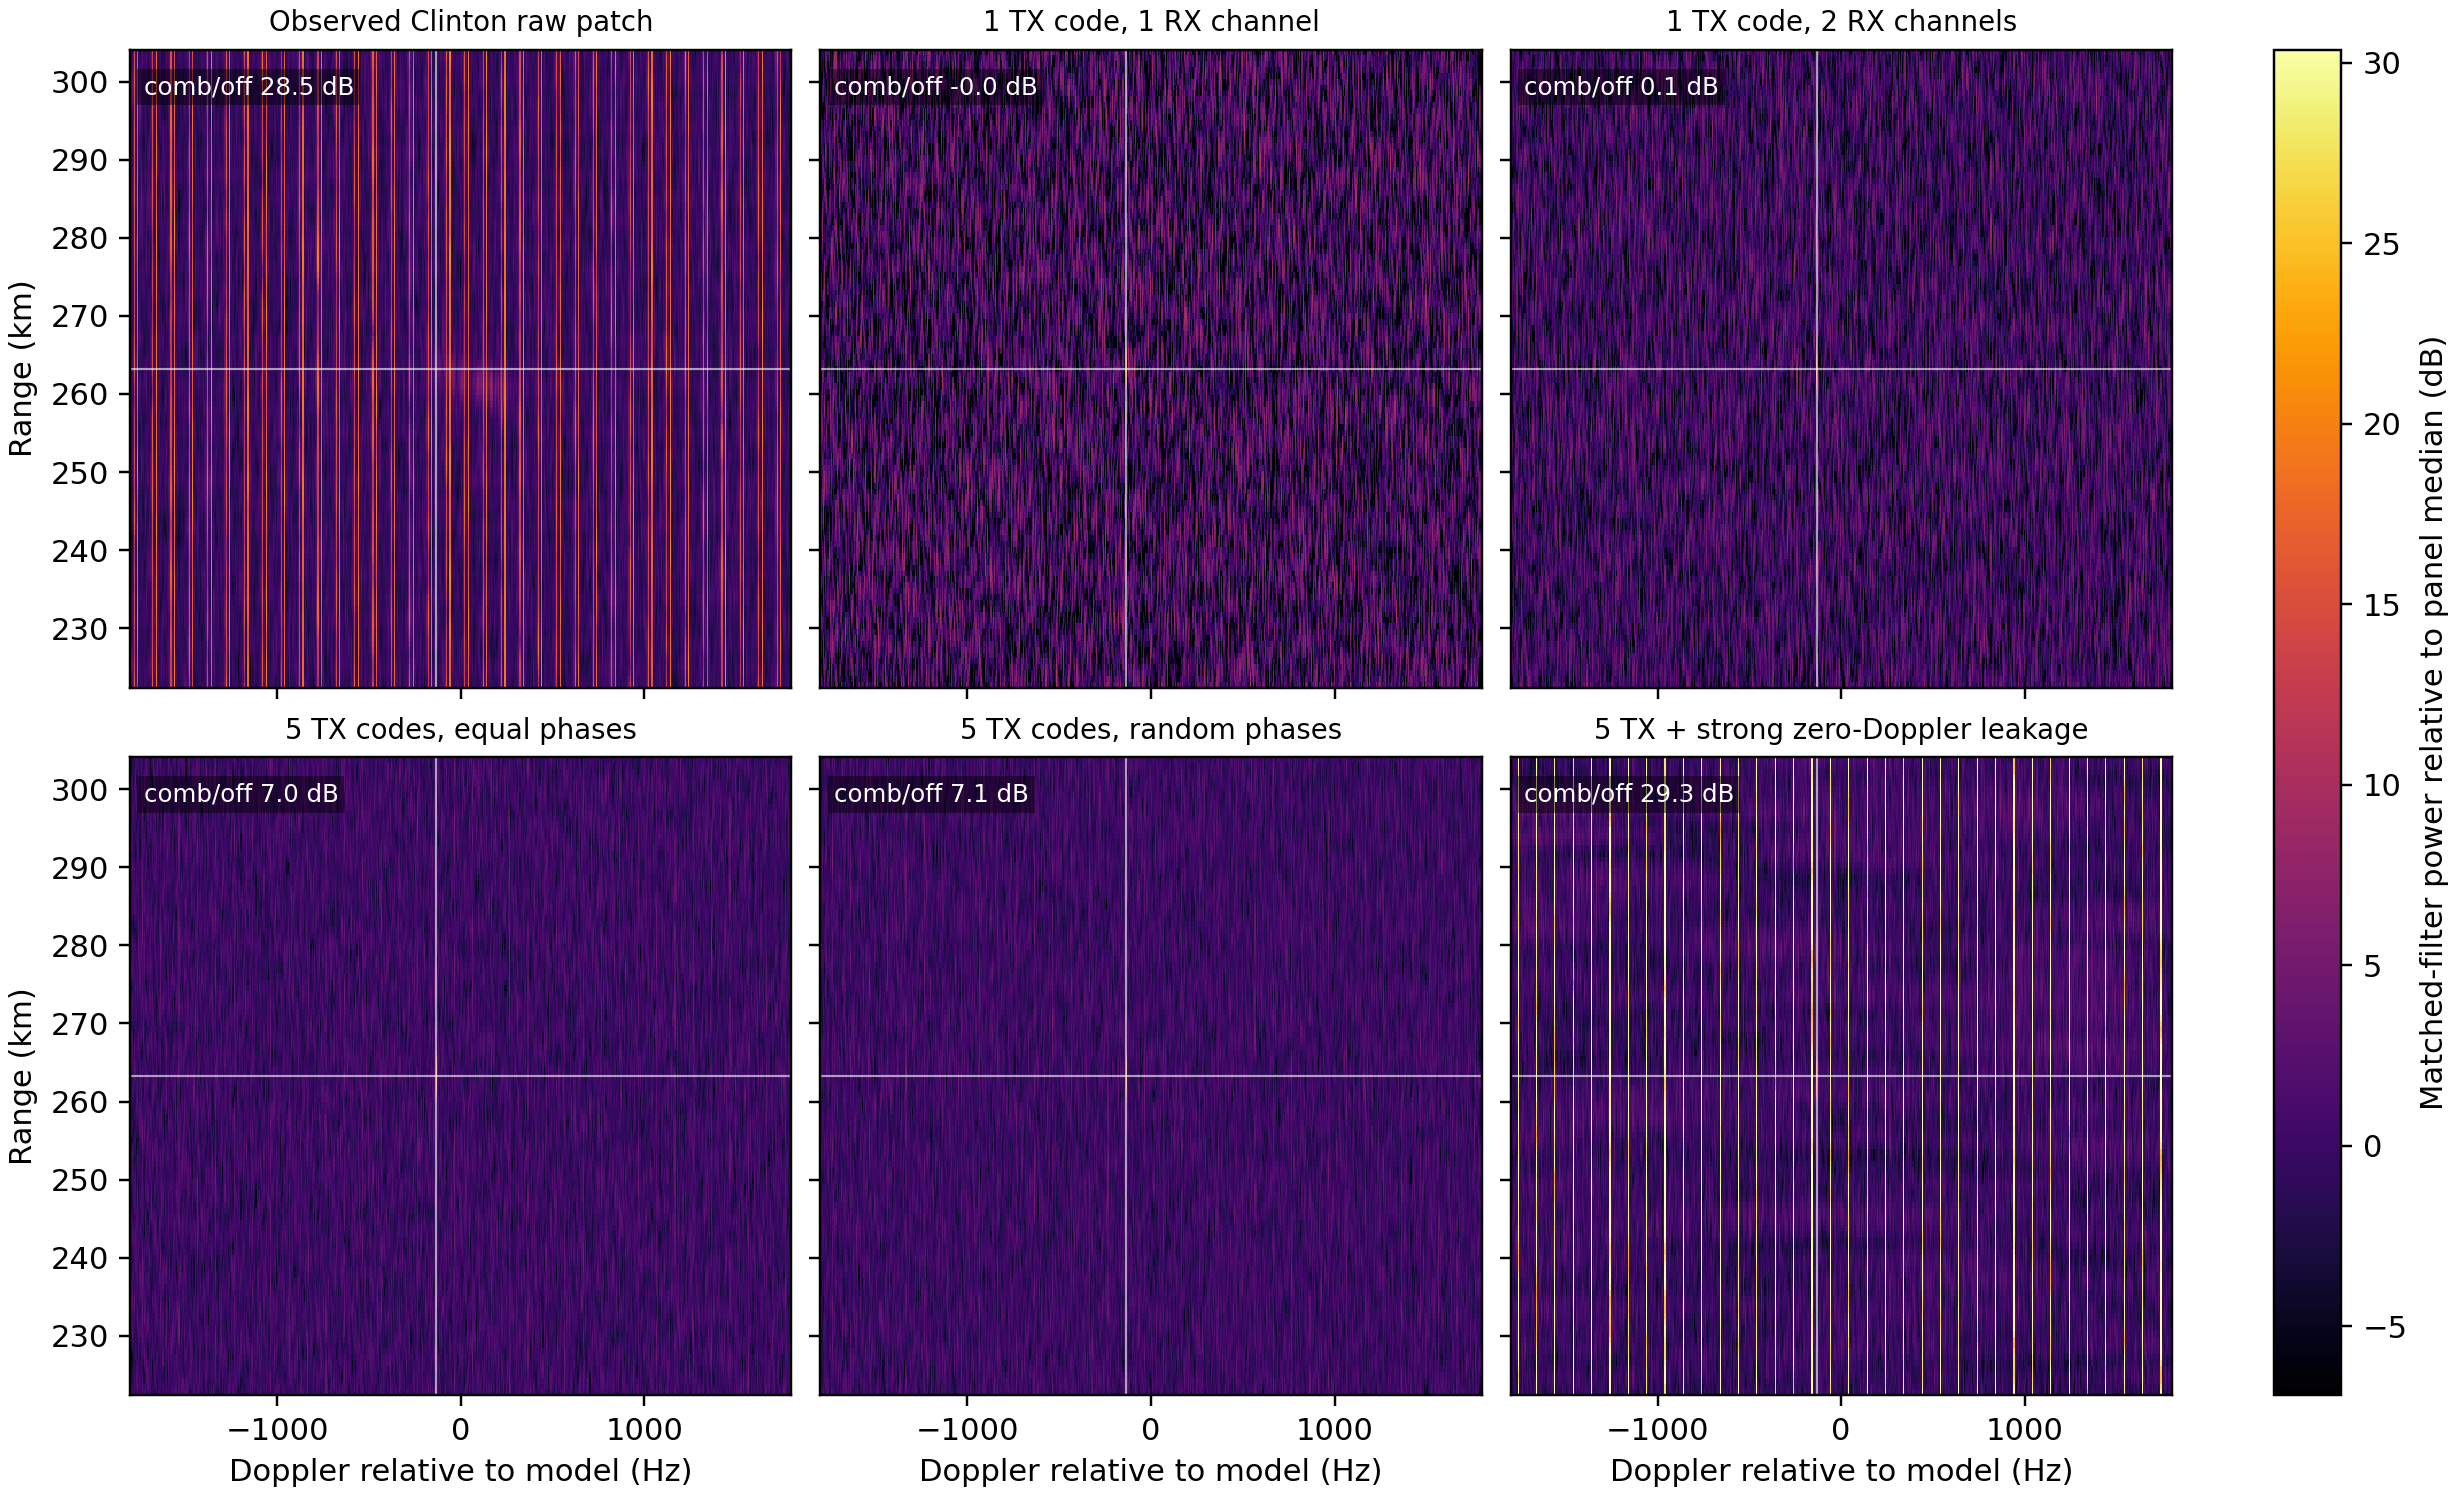
\includegraphics[width=\linewidth]{reports/figures/head_echo_vertical_stripe_simulation.png}
  \caption{Synthetic Clinton matched-filter tests for the vertical stripes in
  the 16-code coherent range--Doppler output.  The first panel is the observed
  raw Clinton patch from Fig.~\ref{fig:head-gaussian-example}.  The remaining
  panels use simulated head echoes with the same range, Doppler shift, matched
  filter grid, and approximate peak-to-background contrast.  White reference
  lines mark the inserted range and Doppler.  Each panel is shown relative to
  its own median matched-filter power.  If the one-code case were already
  stripe dominated, the artifact would be intrinsic to the single repeated-code
  coherent integration.  If the stripes grew only when the other transmitters
  were added, multi-code cross-talk would be implicated.
  \figsource{reports/simulate_head_echo_vertical_stripes.py}}
  \label{fig:head-vertical-stripe-simulation}
\end{figure}

The controlled synthetic point-target cases do not reproduce the observed
vertical stripe pattern as a dominant feature.  Adding the other simultaneously
transmitted code seeds increases the repeated-code comb statistic only modestly
relative to the one-code case, and the 2-D FFT notch strongly suppresses that
image-frequency component.  This argues against ordinary multi-code
cross-correlation of a compact head echo as the sole source of the observed
vertical stripes.  The stress test shows that a strong stationary code-like
leakage term can create more coherent columnar structure, so the next diagnostic
step should be to estimate direct-path and DC-like components together with the
head echo in a sparse range--Doppler model.  In that model the voltage data would
be represented by a sparse set of range--Doppler atoms plus slowly varying
per-range DC or direct-path terms, rather than by subtracting or notching the
matched-filter image after it has already mixed these components.
